% Tipo de documento y tamaño de letra
\documentclass[letterpaper,10pt,twoside,onecolumn]{article}
\textwidth=15cm
% Preparando para documento en Español.
% Para documento en Inglés no hay que hacer esto.
\usepackage[spanish]{babel}
\usepackage{graphicx}
\selectlanguage{spanish}
\usepackage[utf8]{inputenc}
\begin{document}
 
\title{PRODUCTO 5} 
\author{Ana Magdalena Sotomayor} 

\maketitle 
\section{INTRODUCCION}
Se realizaron códigos para graficar en gnuplot los datos para la simulación de un lanzamiento de proyectil o tiro parabólico dado un ángulo de salida y una velocidad inicial dada por el usuario. 
 
Realizamos un código en fortran utilizando la formula de tiro parabólico para obtener los puntos en x y y cada 0.01 segundos y se graficó en gnuplot utilizando datos de entrada para 0grados, 30grados, 60grados y 90grados. 


\section{CODIGOS} 
\subsection{Código Fortran}
\begin{verbatim}
!Programa para obtener los valores cada décima de segundo
!para graficar un tiro parabólico
!Hecho por Ana Sotomayor

program TiroParabolico
   implicit none
   !Definimos variables:
   real, parameter :: pi = 4.0*atan(1.0)
   real ::  vel0, a_grados, rad,  vx, vy, t, h, t2, xtot
   real, parameter :: g = 9.80
   real :: x(4500), y(4500)
   integer :: i
   !Donde vel0 es la velocidad inicial de lanzamiento,
   !a_grados es el ángulo de lanzamiento
   !rad es el ángulo convertido a radianes
   !vx es el componente de la velocidad en x
   !vy es el componente de la velocidad en y
   !h es la altura máxima alcanzada
   !t es el tiempo
   !t2 es el tiempo para llegar a la altura máxima
   !xtot es la distancia total maxima

   !Obtenemos los datos de entrada
   write (*,*) 'Escriba la velocidad inicial en m/s'
   read *,vel0
   write (*,*) 'Escriba el ángulo de tiro del proyectil 
   en grados'
   read *,a_grados
   !Convertimos las velocidades en sus componentes en x y y y 
   los grados a radianes
   rad = a_grados*pi/180
   vx = vel0*cos(rad)
   vy = vel0*sin(rad)
   t = 2*(vy/g)
   h = vy*vy/(2*g)
    
   IF (a_grados == 0 ) THEN
      xtot = 0
     Else  IF (a_grados == 90 ) THEN
      xtot = 0  
     ELSE 
      xtot = vx*t 
   ENDIF   
    !Pantalla de Salida con la información para el usuario.
    write (*,*) 'Con los datos proporcionados de Velocidad',
    vel0,'m/s' 
    write (*,*) 'y un ángulo de lanzamiento de',a_grados, 
    'grados, se calcula que'
    write (*,*) 'El tiempo total de vuelo fue de', t, 'segundos'
    write (*,*) 'La altura maxima alcanzada fue de', h, 'metros'
    write (*,*) 'El alcance maximo del Proyectil fue de', xtot, 
    'metros'

   !Generamos un archivo para almacenar los datos para la simulación
   y los tiempos
   open (1, file = 'simulacion.dat')
   open (2, file = 'Tiempos.dat')
   
   !Generamos las coordenadas del objeto cada décima de segundo)
   do i = 1, 4500, 1
      t = (float(i)*0.01)
      x(i) = vx*t
      y(i) = vy*t - .5*g*t*t
      if (x(i)<0) then
      x(1)=0
      endif 
      write (1,*) x(i), y(i)
      write (2,*) t
      !terminemos el loop cuando el objeto llegue al piso
      if (y(i)<0) exit
   end do
   close (1)
end program TiroParabolico
\end{verbatim}

\subsection{Código para graficar con gnuplot}
\begin{verbatim} 
 set title "Tiro parabolico"
set xlabel "Distancia"
set ylabel "Altura"
set xtics 10.0
set grid 
set xrange [-2:200]
set yrange [0:210]
plot "simulacion.dat" 
pause 5
\end{verbatim}

\subsection{Imagen de salida para 0grados}

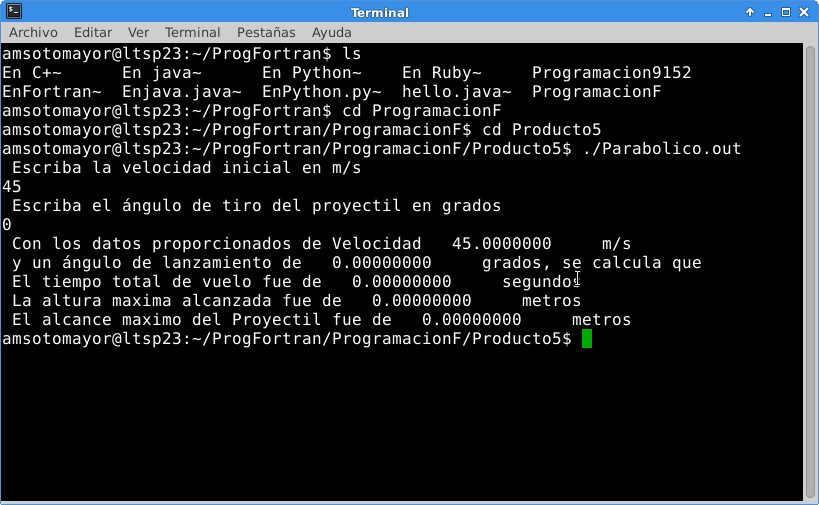
\includegraphics[scale=.40]{salida0g.png}

\subsection{Grafica 0grados}

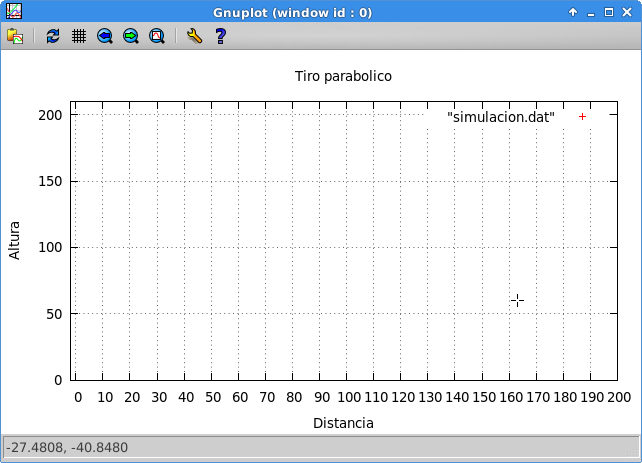
\includegraphics[scale=.50]{grafica0g.png}

\subsection{Imagen de salida para 30grados}

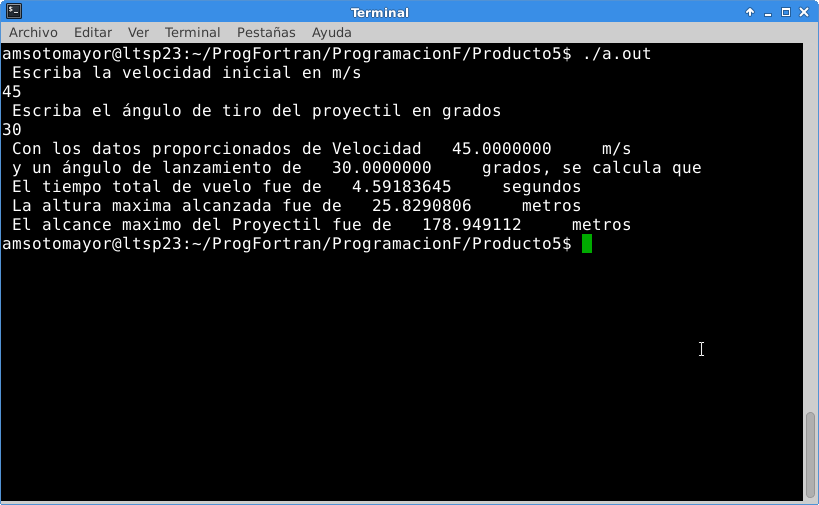
\includegraphics[scale=.40]{salida30g.png}

\subsection{Grafica 30grados}

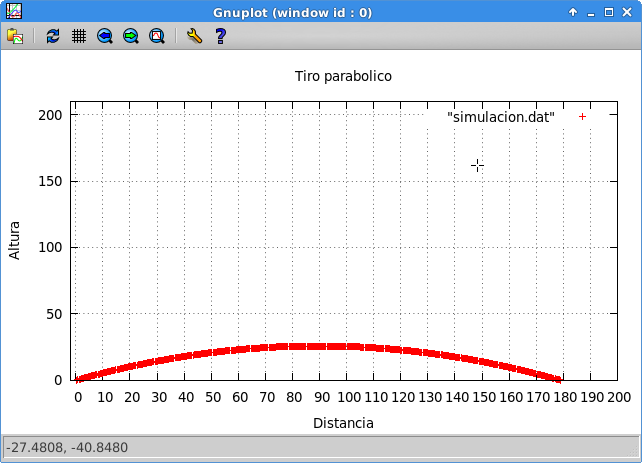
\includegraphics[scale=.50]{Grafica30g.png}

\subsection{Imagen de salida para 60grados}

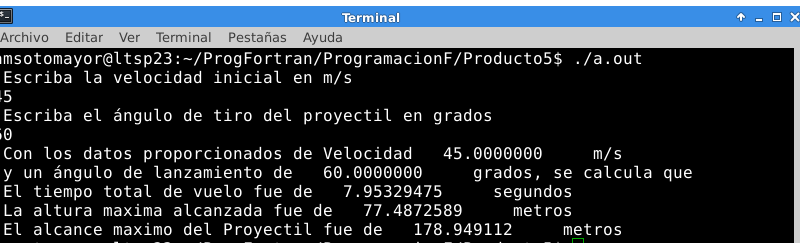
\includegraphics[scale=.40]{salida60g.png}

\subsection{Grafica 60grados}

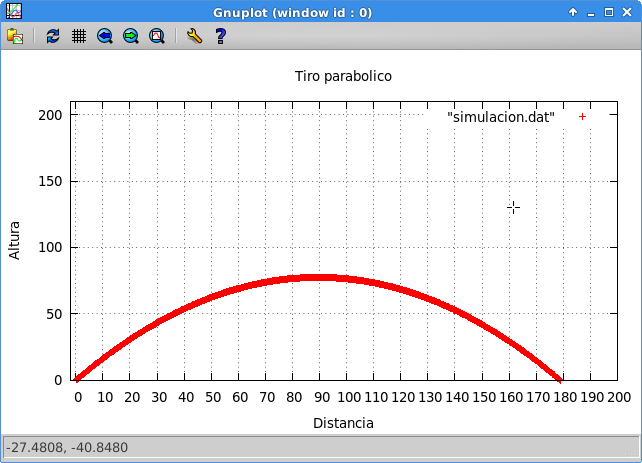
\includegraphics[scale=.50]{grafica60g.png}

\subsection{Imagen de salida para 90grados}

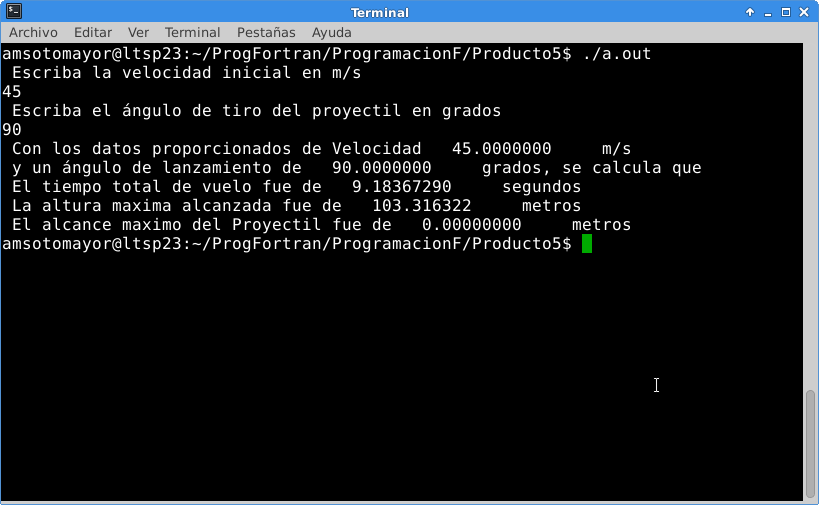
\includegraphics[scale=.40]{Salida90g.png}

\subsection{Grafica 60grados}

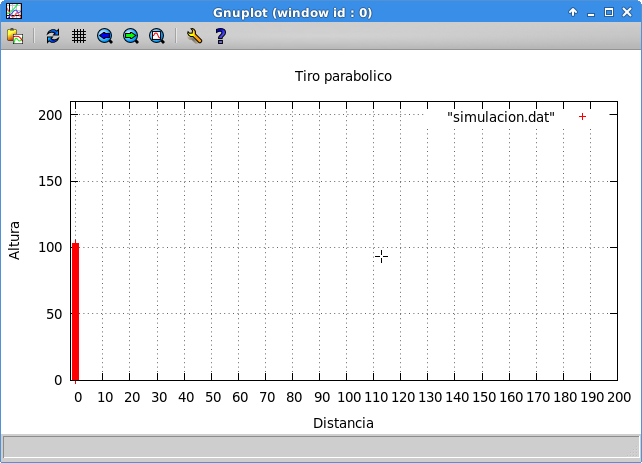
\includegraphics[scale=.50]{grafica90g.png}
% Nunca debe faltar esta ultima linea.
\end{document}